\section{Midterm 2012}

\subsection{Resource Management and Deadlocks}

\begin{example2}{Resource Graph Analysis}\\
    Ein Rechnersystem besitzt zwei Tapestationen (T1, T2) und zwei Disks (D1, D2). Zur Zeit laufen drei Prozesse (P1, P2, P3), wobei folgendes gilt:
    \begin{itemize}
        \item Prozess P1 kopiert Daten von Disk D1 auf die Tapestation T2 und möchte Daten auf den Disk D2 schreiben
        \item Prozess P2 hat Tapestation T1 alloziert und möchte Daten auf Disk D2 schreiben
        \item Prozess P3 hat Disk D2 alloziert und möchte Daten nach Tapestation T2 kopieren
    \end{itemize}
    
    Ist das eine Deadlocksituation, wenn die Ressourcen exklusiv alloziert werden und wenn möchte schreiben das Gleiche wie anfordern bedeutet? Begründen Sie Ihre Antwort (Ressourcengraphen zeichnen und analysieren).
    
    \tcblower
    Ja, dies ist eine Deadlocksituation. 
    
    \textbf{Analyse:}
    \begin{itemize}
        \item P1 hält D1, möchte T2 und D2
        \item P2 hält T1, möchte D2  
        \item P3 hält D2, möchte T2
    \end{itemize}
    
    Es entsteht ein Zyklus: P1 $\rightarrow$ D2 $\rightarrow$ P3 $\rightarrow$ T2 $\rightarrow$ P1\\
    \important{DRAW RESOURCE GRAPH! AND ADD HERE} 
    
    \textbf{Bedingungen für Deadlock:}
    \begin{itemize}
        \item Mutual Exclusion: Ressourcen werden exklusiv alloziert
        \item No Preemption: Ressourcen können nicht weggenommen werden
        \item Hold \& Wait: Prozesse halten Ressourcen und warten auf weitere
        \item Circular Wait: Es gibt einen Zyklus im Ressourcengraph
    \end{itemize}
    
    Alle vier Bedingungen sind erfüllt $\rightarrow$ Deadlock!
\end{example2}

\raggedcolumns

\begin{KR}{Deadlock Detection in Resource Allocation Graphs}
    \paragraph{Resource Graph erstellen}
    \begin{itemize}
        \item Kreise: Prozesse (P1, P2, P3, ...)
        \item Rechtecke: Ressourcen (R1, R2, R3, ...)
        \item Pfeile von Prozess zu Ressource: Reqüst (Anforderung)
        \item Pfeile von Ressource zu Prozess: Allocation (Zuteilung)
    \end{itemize}
    
    \paragraph{Deadlock-Analyse}
    \begin{itemize}
        \item Suche nach Zyklen im Graph
        \item Ein Zyklus bedeutet Deadlock bei Single-Instance Ressourcen
        \item Bei Multi-Instance Ressourcen: Prüfe ob alle Instanzen blockiert
    \end{itemize}
    
    \paragraph{Deadlock-Bedingungen prüfen}
    \begin{itemize}
        \item Mutual Exclusion: Exklusive Ressourcennutzung
        \item Hold \& Wait: Halten und gleichzeitig warten
        \item No Preemption: Keine Unterbrechung möglich
        \item Circular Wait: Zyklische Warteabhängigkeiten
    \end{itemize}
    
    \paragraph{Lösungsansätze}
    \begin{itemize}
        \item Prevention: Eine der vier Bedingungen verhindern
        \item Avoidance: Banker's Algorithm
        \item Detection \& Recovery: Deadlock erkennen und auflösen
    \end{itemize}
\end{KR}

\subsection{Synchronization with Semaphores}

\begin{example2}{Semaphore Implementation}\\
    Gegeben sind drei Prozess P0, P1, und P2 die nach folgendem Schema abgearbeitet werden soll:\\
    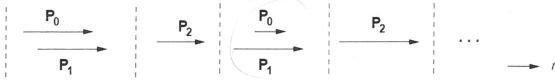
\includegraphics[width=\linewidth]{semaphore_mt12.png}
    \begin{center}
    P0 $\rightarrow$ P2 $\rightarrow$ P0 $\rightarrow$ P2 $\rightarrow$ ...\\
    P1 (parallel)
    \end{center}
    
    Die Verarbeitung startet mit den beiden Prozessen P0 und P1, die parallel verarbeitet werden sollen (es spielt kein Rolle, welcher der beiden Prozesse zürst mit seiner Verarbeitung beginnt oder aufhört). Wenn beide Prozesse eine Iteration ihrer Funktion working(x) beendet haben, folgt Prozess P2, etc.
    
    Schreiben Sie Pseudocode mit maximal 3 Semaphoren S0, S1 und S3, der garantiert, dass die oben skizzierte Reihenfolge eingehalten wird. Verwenden Sie dazu ausschliesslich Befehle der Form up(S0) und down(S0), etc. Geben Sie an, wie die Semaphore initialisiert werden müssen.
    
    \tcblower
    \important{ABGLEICHEN MIT LÖSUNG UND BESSER FORMATIEREN}
    \begin{center}
    \begin{tabular}{|c|c|c|}
    \hline
    \textbf{P0} & \textbf{P1} & \textbf{P2} \\
    \hline
    Sem S0: 1 & Sem S1: 1 & Sem S2: 0 \\
    Sem S3: 0 & Sem S3: 0 & \\
    \hline
    while(1) \{ & while(1) \{ & while(1) \{ \\
    \quad down(S0); & \quad down(S1); & \quad down(S2); \\
    \quad working(0); & \quad working(1); & \quad working(2); \\
    \quad up(S3); & \quad up(S3); & \quad up(S0); \\
    \} & \} & \quad up(S1); \\
     &  & \} \\
    \hline
    \end{tabular}
    \end{center}
    
    \textbf{Initialisierung:}
    \begin{itemize}
        \item S0 = 1 (P0 kann starten)
        \item S1 = 1 (P1 kann starten) 
        \item S2 = 0 (P2 muss warten)
        \item S3 = 0 (Synchronisation zwischen P0/P1 und P2)
    \end{itemize}
    
    \textbf{Ablauf:}
    \begin{itemize}
        \item P0 und P1 starten parallel
        \item Beide signalisieren mit up(S3) wenn fertig
        \item P2 wartet mit down(S2) bis beide P0 und P1 fertig sind
        \item P2 gibt mit up(S0) und up(S1) die nächste Runde frei
    \end{itemize}
\end{example2}

\begin{KR}{Semaphore-basierte Synchronisation}
    \paragraph{Semaphore verstehen}
    \begin{itemize}
        \item Semaphore S ist ein Zähler mit atomaren Operationen
        \item down(S) oder P(S): Dekrementiert S, blockiert bei S $\leq$  0
        \item up(S) oder V(S): Inkrementiert S, weckt wartende Prozesse
        \item Initialisierung bestimmt verfügbare Ressourcen
    \end{itemize}
    
    \paragraph{Synchronisationsmuster}
    \begin{itemize}
        \item Mutual Exclusion: Binary Semaphore (0/1) um kritische Bereiche
        \item Signaling: Ein Prozess signalisiert einem anderen (Producer-Consumer)
        \item Rendezvous: Zwei Prozesse warten aufeinander
        \item Barrier: Mehrere Prozesse warten aufeinander
    \end{itemize}
    
    \paragraph{Typische Synchronisationsprobleme}
    \begin{itemize}
        \item Producer-Consumer: Buffer-Management mit vollen/leeren Plätzen
        \item Reader-Writer: Mehrere Leser oder ein Schreiber
        \item Dining Philosophers: Deadlock-Vermeidung bei zyklischen Abhängigkeiten
        \item Barrier Synchronization: Alle warten aufeinander
    \end{itemize}
    
    \paragraph{Implementierungsschritte}
    \begin{itemize}
        \item Identifiziere Synchronisationspunkte
        \item Bestimme benötigte Semaphore und deren Initialisierung
        \item Verwende down() vor kritischen Bereichen/Warten
        \item Verwende up() nach kritischen Bereichen/Signaling
        \item Teste auf Deadlock-Freiheit und korrekte Reihenfolge
    \end{itemize}
\end{KR}

\subsection{Memory Management}

\begin{example2}{Buddy System}\\
    Ein Betriebssystem-Kernel verwaltet seine Datenbuffer mit einem Buddy System, wobei insgesamt 8MByte Speicher zur Verfügung stehen. Zur Zeit sind folgende Buffer mit 62KByte, 34KByte und 9KByte alloziert worden. Wie viel Speicher geht dabei durch interne Fragmentierung insgesamt verloren, Angabe in KByte:
    
    \tcblower
    \begin{minipage}{0.5\linewidth}
    Buddy System alloziert in Potenzen von 2:
    
    \begin{itemize}
        \item 62 KByte $\rightarrow$ nächste 2er-Potenz: 64 KByte
        \item 34 KByte $\rightarrow$ nächste 2er-Potenz: 64 KByte  
        \item 9 KByte $\rightarrow$ nächste 2er-Potenz: 16 KByte
    \end{itemize}
    \end{minipage}
    \begin{minipage}{0.5\linewidth}
    Interne Fragmentierung = Alloziert - Angefordert:
    \begin{itemize}
        \item (64 - 62) = 2 KByte
        \item (64 - 34) = 30 KByte
        \item (16 - 9) = 7 KByte
    \end{itemize}
    \end{minipage}
    \vspace{2mm}\\
    Gesamt: 2 + 30 + 7 = \textbf{39 KByte} interne Fragmentierung
\end{example2}

\begin{example2}{Page Tables}\\
    Ein Prozessor besitzt eine Wortbreite von 32Bit. Pointer (Adressen) werden in 32Bit Worten gespeichert, aber nur die 24 tieferwertigen Bits werden für die Adressbildung verwendet (Bits 25-31sind auf 0 gesetzt).
    
    Die logische Adresse ist wie folgt strukturiert:
    \begin{center}
    \begin{tabular}{|c|c|c|}
    \hline
    6-Bit Page Directory & 8-Bit Page Nummer & 10-Bit Offset \\
    \hline
    \end{tabular}
    \end{center}
    
    a) Wie gross ist eine Page, Angabe in KBytes?\\
    b) Wie viele Bytes enthält das Page Directory, wenn pro Eintrag ein Pointer (Adresse) auf eine Page Tabelle eingetragen wird, Angabe in KBytes?\\
    c) Wie viele Page Tabellen kann ein Prozess maximal haben?\\
    d) Wie viele Frames kann das System maximal haben?
    
    \tcblower
    \begin{minipage}{0.5\linewidth}
    \textbf{Lösung:}
    
    a) Page-Grösse = 2\textsuperscript{10} Bit = 1024 Bytes = \textbf{1 KByte}
    
    b) Page Directory:
    \begin{itemize}
        \item 6 Bit $\rightarrow$ 2\textsuperscript{6} = 64 Einträge
        \item 4 Bytes pro Adresse
        \item 64 × 4 = 256 Bytes = \textbf{0.25 KBytes}
    \end{itemize}
    \end{minipage}
    \begin{minipage}{0.5\linewidth}    
    c) Page Tabellen: 6 Bit $\rightarrow$ 2\textsuperscript{6} = \textbf{64 Page Tabellen}
    
    d) Frames im System:
    \begin{itemize}
        \item 24 Bit physische Adresse
        \item 10 Bit Offset pro Frame
        \item Frame-Bits: 24 - 10 = 14 Bit
        \item Maximale Frames: 2\textsuperscript{14} = \textbf{16384 Frames}
    \end{itemize}
    \end{minipage}
\end{example2}



\begin{KR}{Memory Management Analysis}
    \paragraph{Buddy System}
    \begin{itemize}
        \item Alloziert in Potenzen von 2 (1, 2, 4, 8, 16, ... KByte)
        \item Interne Fragmentierung = Alloziert - Angefordert
        \item Nächste grössere 2er-Potenz finden: 2\textsuperscript{n} $\geq$ Anforderung
        \item Beispiel: 33 KByte $\rightarrow$ 64 KByte (2\textsuperscript{6})
    \end{itemize}
    
    \paragraph{Page Table Berechnung}
    \begin{itemize}
        \item Page-Grösse = 2\textsuperscript{Offset-Bits} Bytes
        \item Anzahl Pages = 2\textsuperscript{Page-Number-Bits}
        \item Page Directory Grösse = 2\textsuperscript{Directory-Bits} × Pointer-Grösse
        \item Maximale Frames = 2\textsuperscript{(Physische-Adress-Bits - Offset-Bits)}
    \end{itemize}
    
    \paragraph{Adressaufteilung}
    \begin{itemize}
        \item Logische Adresse = Page Directory + Page Number + Offset
        \item Physische Adresse = Frame Number + Offset
        \item Page Table Entry enthält Frame Number
        \item Translation: Page Number $\rightarrow$ Frame Number
    \end{itemize}
    
    \paragraph{Memory Hierarchie}
    \begin{itemize}
        \item Page Directory zeigt auf Page Tables
        \item Page Tables zeigen auf Frames
        \item Mehrstufige Page Tables reduzieren Speicherbedarf
        \item TLB cached häufig verwendete Translations
    \end{itemize}
\end{KR}

\subsection{Page Replacement Algorithms}

\begin{example2}{Least Recently Used (LRU)}\\
    Ein Prozess referenziert der Reihe nach folgende Pages:
    \begin{center}
    8 7 5 8 7 3 5 1 3 4 2 1 8 3 1 2
    \end{center}
    
    Gehen Sie davon aus, dass zu Beginn keine Pages im Speicher stehen und dass auch das erstmalige Laden einer Page als Page Fault gezählt wird (demand paging). Pro Prozess stehen 4 Frames zur Verfügung.
    
    Tragen Sie in unten stehender Tabelle die den Frames zugewiesenen Pages für den Least Recently Used Algorithmus. Das Page mit diesem Zugriff am weitesten zurückliegend wird dann mit ein neüs Page ersetzt.
    
    Markieren Sie die Spalten mit einem Stern, wo ein Page Fault auftritt. Nehmen Sie an, dass ausschliesslich Demand Paging verwendet wird. Wenn mehrere Frames für das placement resp. replacement in Frage kommen, muss der Frame mit der kleinsten Nummer gewählt werden.
    
    \tcblower
    
    \textbf{Lösung:}
    
    \begin{center}
    \begin{tabular}{|l|c|c|c|c|c|c|c|c|c|c|c|c|c|c|c|c|}
    \hline
    Referenzen & 8 & 7 & 5 & 8 & 7 & 3 & 5 & 1 & 3 & 4 & 2 & 1 & 8 & 3 & 1 & 2 \\
    \hline
    frame 1 & 8* & 8 & 8 & 8 & 8 & 8 & 8 & 1* & 1 & 1 & 1 & 1 & 1 & 1 & 1 & 1 \\
    \hline
    frame 2 & & 7* & 7 & 7 & 7 & 7 & 7 & 7 & 7 & 4* & 4 & 4 & 8* & 8 & 8 & 8 \\
    \hline
    frame 3 & & & 5* & 5 & 5 & 5 & 5 & 5 & 5 & 5 & 2* & 2 & 2 & 2 & 2 & 2 \\
    \hline
    frame 4 & & & & & & 3* & 3 & 3 & 3 & 3 & 3 & 3 & 3 & 3 & 3 & 3 \\
    \hline
    page fault & × & × & × & & & × & & × & & × & × & & × & & & \\
    \hline
    \end{tabular}
    \end{center}
    
    \textbf{Page Faults:} 8 von 16 Zugriffen
    
    \textbf{LRU-Logik:}
    \begin{itemize}
        \item Bei jedem Zugriff wird die "letzte Verwendung" der Page aktualisiert
        \item Bei einem Page Fault wird die am längsten nicht verwendete Page ersetzt
        \item Zeitstempel oder Zugriffs-Historie bestimmen LRU-Page
    \end{itemize}
\end{example2}

\begin{KR}{Page Replacement Algorithms}
    \paragraph{Least Recently Used (LRU)}
    \begin{itemize}
        \item Ersetze die Page, die am längsten nicht verwendet wurde
        \item Gute Performance, aber aufwändig zu implementieren
        \item Benötigt Zeitstempel oder Zugriffs-Historie
        \item Approximation durch Clock Algorithm oder Second Chance
    \end{itemize}
    
    \paragraph{First-In-First-Out (FIFO)}
    \begin{itemize}
        \item Ersetze die älteste Page (first loaded)
        \item Einfach zu implementieren mit Qüü
        \item Kann zu Belady's Anomaly führen
        \item Nicht optimal, da alte Pages oft noch verwendet werden
    \end{itemize}
    
    \paragraph{Optimal (OPT)}
    \begin{itemize}
        \item Ersetze Page, die am spätesten wieder verwendet wird
        \item Theoretisch optimal, praktisch nicht implementierbar
        \item Benötigt Zukunftswissen über Page-Zugriffe
        \item Wird als Benchmark für andere Algorithmen verwendet
    \end{itemize}
    
    \paragraph{Implementation Tips}
    \begin{itemize}
        \item Page Fault tritt auf bei erstem Zugriff auf neü Page
        \item Bei mehreren Kandidaten: Wähle Frame mit kleinster Nummer
        \item Clock Algorithm: Circular list mit Reference Bit
        \item Working Set: Berücksichtige lokale vs. globale Ersetzung
    \end{itemize}
\end{KR}

\subsection{Operating System Concepts}

\begin{example2}{Multiple Choice Qüstions}\\
    Pro Teilfrage können eine, mehrere oder keine Antworten zutreffen, kreuzen Sie die richtige(n) Antwort(en) an.
    
    a) Welche der folgenden Aussagen treffen zu?
    \begin{itemize}
        \item[\textcolor{frog}{$\checkmark$}] Alle Mutexes können mit Semaphoren realisiert werden
        \item[\textcolor{red}{$\times$}] Semaphore können in allen Fällen durch Mutexes ersetzt werden  
        \item[\textcolor{red}{$\times$}] Mutexes sollten immer anstelle von Semaphoren eingesetzt werden, weil es dann keine Deadlocks geben kann
        \item[\textcolor{frog}{$\checkmark$}] Mit Semaphoren lässt sich die Verarbeitungsreihenfolge von Prozessen und Threads erzwingen
    \end{itemize}
    
    b) Welcher der folgenden Aussagen treffen zu?
    \begin{itemize}
        \item[\textcolor{red}{$\times$}] Pages müssen grösser als Frames dimensioniert werden
        \item[\textcolor{red}{$\times$}] Es müssen mindestens so viele Pages wie Frames in einem System vorhanden sein
        \item[\textcolor{red}{$\times$}] Sowohl interne wie auch externe Fragmentierung treten bei Paging auf
        \item[\textcolor{frog}{$\checkmark$}] Pages und Frames müssen gleich gross dimensioniert werden
    \end{itemize}
    
    c) Welcher der folgenden Aussagen treffen zu?
    \begin{itemize}
        \item[\textcolor{frog}{$\checkmark$}] Ein MMU übersetzt Logischen Adressen zu Physikalische Adressen
        \item[\textcolor{red}{$\times$}] Swap in bedeutet dass ein Prozess auf die Hard-Disk verlagert wird
        \item[\textcolor{red}{$\times$}] Ein Prozess der auf der Harddisk verlagert worden ist kann sich im Zustand Running befinden
    \end{itemize}
    
    d) Welcher der folgenden Aussagen treffen zu?
    \begin{itemize}
        \item[\textcolor{red}{$\times$}] Bei Static Partitioning tritt External Fragmentation auf
        \item[\textcolor{frog}{$\checkmark$}] Bei Dynamic Partitioning tritt External Fragmentation auf  
        \item[\textcolor{red}{$\times$}] Nur bei Best Fit Allocation wird kein Compaction benötigt
    \end{itemize}
    
    \tcblower
    
    \textbf{Erklärungen:}
    
    a) Semaphore vs. Mutexes:
    \begin{itemize}
        \item[\textcolor{frog}{$\checkmark$}] Mutexes sind Binary Semaphores (0/1) - können mit Semaphoren realisiert werden
        \item[\textcolor{red}{$\times$}] Counting Semaphores (>1) können nicht durch Mutexes ersetzt werden
        \item[\textcolor{red}{$\times$}] Auch mit Mutexes sind Deadlocks möglich
        \item[\textcolor{frog}{$\checkmark$}] Semaphore eignen sich gut für Prozess-Synchronisation
    \end{itemize}
    
    b) Paging:
    \begin{itemize}
        \item[\textcolor{red}{$\times$}] Pages und Frames sind gleich gross
        \item[\textcolor{red}{$\times$}] Anzahl ist unabhängig - Virtual Memory ermöglicht mehr Pages als Frames
        \item[\textcolor{red}{$\times$}] Nur interne Fragmentierung (innerhalb Pages)
        \item[\textcolor{frog}{$\checkmark$}] Pages (logisch) = Frames (physisch) in der Grösse
    \end{itemize}
    
    c) Memory Management:
    \begin{itemize}
        \item[\textcolor{frog}{$\checkmark$}] MMU (Memory Management Unit) macht Address Translation
        \item[\textcolor{red}{$\times$}] Swap in = von Disk in Memory (nicht umgekehrt)
        \item[\textcolor{red}{$\times$}] Ausgelagerte Prozesse sind nicht Running
    \end{itemize}
    
    d) Partitioning:
    \begin{itemize}
        \item[\textcolor{red}{$\times$}] Static: Interne Fragmentierung (feste Grössen)
        \item[\textcolor{frog}{$\checkmark$}] Dynamic: Externe Fragmentierung (variable Grössen)
        \item[\textcolor{red}{$\times$}] Alle Dynamic Allocation Methoden benötigen eventüll Compaction
    \end{itemize}
\end{example2}

\begin{KR}{Operating System Core Concepts}
    \paragraph{Synchronisation Mechanisms}
    \begin{itemize}
        \item Mutex: Binary lock (0/1) für kritische Bereiche
        \item Semaphore: Counting mechanism für Resource Management
        \item Monitor: High-level synchronization construct
        \item Condition Variables: Wait/Signal mechanism
    \end{itemize}
    
    \paragraph{Memory Management}
    \begin{itemize}
        \item Pages: Logische Memory-Einheiten (Virtual Memory)
        \item Frames: Physische Memory-Einheiten (Physical Memory)  
        \item MMU: Hardware für Address Translation
        \item TLB: Cache für Address Translation
    \end{itemize}
    
    \paragraph{Process States und Swapping}
    \begin{itemize}
        \item Running: Prozess auf CPU
        \item Ready: Bereit zur Ausführung
        \item Blocked: Wartet auf I/O oder Resource
        \item Swapped: Auf Disk ausgelagert (nicht Ready/Running)
    \end{itemize}
    
    \paragraph{Memory Allocation}
    \begin{itemize}
        \item Static Partitioning: Feste Grössen $\rightarrow$ Interne Fragmentierung
        \item Dynamic Partitioning: Variable Grössen $\rightarrow$ Externe Fragmentierung
        \item Paging: Feste Page/Frame Grösse $\rightarrow$ Nur interne Fragmentierung
        \item Compaction: Löst externe Fragmentierung durch Memory-Reorganisation
    \end{itemize}
\end{KR}

\begin{remark}
    Diese Exam-Beispiele decken die wichtigsten Konzepte des Betriebssystem-Kurses ab:
    \begin{itemize}
        \item Deadlock Detection und Resource Management
        \item Process Synchronization mit Semaphoren
        \item Memory Management (Buddy System, Paging)
        \item Page Replacement Algorithms
        \item Grundlegende OS-Konzepte
    \end{itemize}
    Die KRs bieten systematische Herangehensweisen für ähnliche Aufgaben in Prüfungen.
\end{remark}